\documentclass{article}
\usepackage{amsmath}
\usepackage{graphicx} % Required for inserting images

\title{Assignment 1 Writeup}

\begin{document}

\setlength{\parindent}{0pt}
\setlength{\parskip}{\baselineskip}

\maketitle

\section{Program 1}
The speedup for 2-8 threads for each view is below.

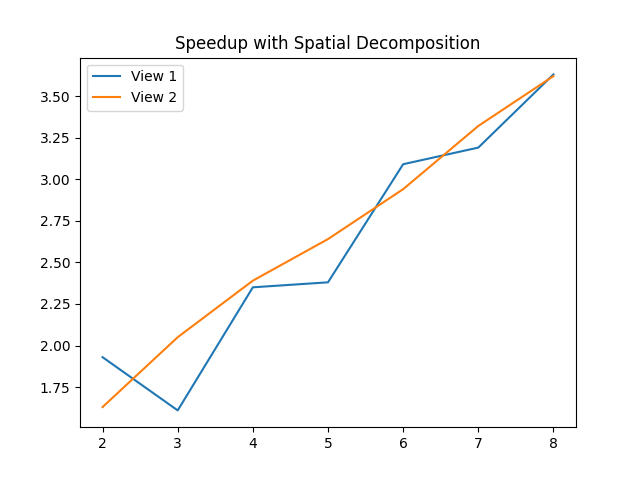
\includegraphics[width=1\textwidth]{speedup_spatial.png}

The dip at three threads is likely due to the uneven work distribution -- the
``middle'' thread has more than 50\% of the work to do. Contrast with View 2,
which has a much more even distribution when decomposed spatially and hence
does not show this patter. In general, we don't get 1:1 speedups as threads
increase due to uneven work distribution.

The timings, shown below, bear this out.

\begin{center}
\begin{tabular}{ l r r r }
  Threads & t0 & t1 & t2 \\
  2 & 213.021 & 213.300 & \\
  3 & 86.072  & 257.164 & 86.621
\end{tabular}
\end{center}

To solve this problem, we can interleave the rows across threads such that
$\mathrm{thread}_{i}$ processes all rows where {\tt rownum \% i == 0}. This
should produce a much more even work distribution. Figure 2 shows speedups with
this policy.

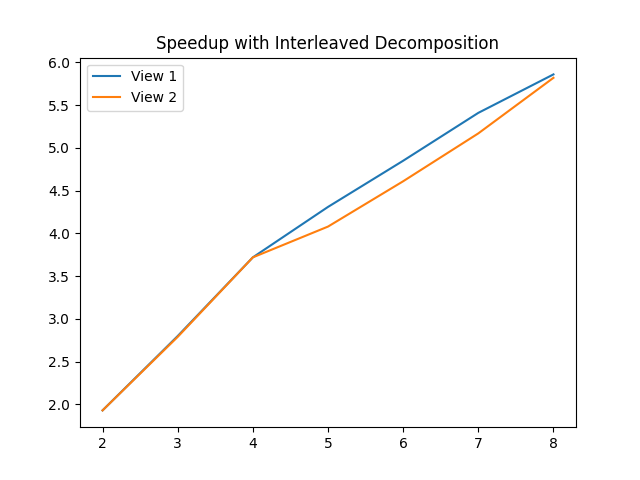
\includegraphics[width=1\textwidth]{speedup_interleaved.png}

Increasing to 16 threads does not have a useful effect as after 8 threads, all
cores are fully utilized, so any additional threads will have to wait. There is
also a context switching overhead.

\end{document}
